\section{Pixel-Space Video Forecasting Pilot}\label{app:video-case}
We extend the conditional forecast models to KTH human actions and CLEVRER object-motion videos, following the video tasks of \citet{chen2024forecasting}. This pilot generates pixels directly, without a latent autoencoder, and conditions on the last $N$ consecutive frames. Every generated frame enters its own ensemble member's rolling history; later observed frames are used only for evaluation. KTH uses grayscale images and $10$ observed frames followed by $30$ forecasts. CLEVRER uses RGB images, two observed frames and $14$ forecasts, retaining every fifth original frame. Both datasets are processed at $64\times64$ pixels. For CLEVRER, this deliberately reduces the $128\times128$ resolution of the audited RIVER reference configuration.\footnote{\href{https://github.com/Araachie/river/blob/9ecde339e4c19713485fc1ab31bcb524d6772f6e/configs/clevrer.yaml}{Pinned CLEVRER reference configuration}. The released forecasting demo contains inconsistent spatial declarations; this pilot does not claim an exact numerical reproduction.}

\begin{table*}[t]
\centering
\small
\input{figures/video_case/setup_table}
\caption{Pixel-video setup. $N$ is observed history length and $L$ is the number of future frames; stride counts original video frames. Counts are annotated segments for KTH and videos for CLEVRER. KTH uses subjects 1--18 for training, 19--20 for validation, and 21--25 for testing. CLEVRER retains its official splits. Each dataset has 128 frozen, sufficiently long test cases and four completions per case.}
\label{tab:video-setup}
\end{table*}

All four model families are trained separately on each dataset. The stochastic-interpolant and flow-matching teachers start from random initialization; each map starts from its own newly trained video teacher. No Navier--Stokes weights are reused. A shared conditional U-Net has widths $(16,32,64)$ and a 128-dimensional time embedding; the fixed history is concatenated along channels. Teachers receive 20,000 updates at batch size 16. Map training uses 2,000 progressive-distillation updates and 500 teacher-rollout refinement updates, with 32 teacher evaluations per supervised interval. The It\^o map retains four path increments per pixel channel. Refinement retains the diagonal loss and samples intervals over the full range, including a probability-$0.5$ atom at $[0,1]$. Fixed-noise validation selects each stage's checkpoint before test evaluation.

\begin{table*}[t]
\centering
\small
\input{figures/video_case/training_table}
\caption{Completed training and frozen evaluation budgets. ``Own updates'' excludes a map's already trained teacher: each map additionally depends on its corresponding 20,000-update teacher. Parameter counts come from the archived trained configurations. Test NFEs are neural evaluations per generated frame and per member; both listed budgets use the same selected checkpoint. These training and architecture counts are not forecast-quality results.}
\label{tab:video-training}
\end{table*}

\begin{figure*}[t]
\centering
\includegraphics[width=\textwidth]{figures/video_case/dataset_previews.pdf}
\caption{Observed dataset examples after pixel preprocessing; \emph{these are not model forecasts}. KTH panels show different clips from the six action classes, rather than successive times of one trajectory. CLEVRER panels show one observed clip at original frame indices $0,5,10,25,50,75$, corresponding to retained-frame indices $0,1,2,5,10,15$. Images were fixed during dataset preparation, before model evaluation.}
\label{fig:video-dataset-preview}
\end{figure*}

The frozen evaluation compares map budgets $1,8$ with solver budgets $16,64$ and a persistence baseline on identical cases. FVD uses the same pretrained 400-dimensional I3D detector for every model and embeds observed context followed by the generated future. We report 128 real versus 512 generated clips, together with four equal-count 128-versus-128 FVD values, one for each completion index. This differs from the much larger completion count in \citet{chen2024forecasting}; no latent-reconstruction correction is applied. Future-only diagnostics include fair CRPS and energy score, ensemble-mean RMSE, spread/coverage, PSNR, SSIM and LPIPS. Source-video grouping accounts for multiple KTH segments from one original video. Image metrics and display clip their copies to the pixel range, while autoregressive feedback and proper scores retain unmodified predictions.

All eight dataset/model combinations have completed training, and checkpoint hashes, metric weights and test cases were frozen before held-out evaluation. Training wall times include periods of shared GPU use with the separately requested stability study. Video sampling-time comparisons use GPU-exclusive evaluation.

\IfFileExists{generated/video_results.tex}{%
\subsection{Held-Out Pixel-Video Results}\label{app:video-results}

Both frozen video evaluations and their artifact audits are complete. Results below use all four model families and persistence on the same cases; this single-training-seed pixel pilot is not a reproduction of the larger latent-space benchmark.

Frame scores average over future leads and weight original source videos equally. FVD uses the selected clip distribution. Time is generation seconds for a complete four-member rollout, and rollout NFE counts neural calls per member over all future frames. Member-FVD SD measures completion randomness, not uncertainty over test cases or training seeds. SI denotes the stochastic interpolant and FM denotes flow matching.

\begin{table*}[t]\centering\small

\begin{tabular}{lrrrrrr}
\toprule
Model & Steps/frame & Rollout NFE & Time (s)$\downarrow$ & CRPS$\downarrow$ & FVD pooled$\downarrow$ & FVD member mean $\pm$ SD \\
\midrule
SI & 16 & 224 & 1.47 & 0.0107 & 436.1 & 485.3 $\pm$ 16.2 \\
SI & 64 & 896 & 5.81 & 0.0094 & 222.3 & 268.9 $\pm$ 10.7 \\
FM & 16 & 224 & 1.45 & 0.0098 & 323.0 & 361.8 $\pm$ 19.1 \\
FM & 64 & 896 & 5.81 & 0.0096 & 330.0 & 372.1 $\pm$ 19.8 \\
It\^o map & 1 & 14 & 0.13 & 0.0140 & 1080.0 & 1117.4 $\pm$ 18.9 \\
It\^o map & 8 & 112 & 0.99 & 0.0110 & 317.3 & 360.5 $\pm$ 6.0 \\
Flow map & 1 & 14 & 0.10 & 0.0110 & 402.2 & 442.7 $\pm$ 5.4 \\
Flow map & 8 & 112 & 0.80 & 0.0101 & 320.4 & 359.9 $\pm$ 15.3 \\
Persistence & 1 & 0 & 0.00 & 0.0107 & 1072.2 & 1071.5 $\pm$ 0.0 \\
\bottomrule
\end{tabular}


\caption{CLEVRER: matched pilot distributional quality and generation cost. Pooled FVD uses 128 real and 512 generated clips; member FVD uses 4 separate 128-versus-128 comparisons. Lower CRPS and FVD are better. Persistence has zero neural evaluations.}\label{tab:video-clevrer-quality}

\end{table*}

\begin{table*}[t]\centering\small

\begin{tabular}{lrrrrrr}
\toprule
Model & Steps/frame & Sample PSNR$\uparrow$ & Sample SSIM$\uparrow$ & Sample LPIPS$\downarrow$ & Mean PSNR$\uparrow$ & Mean SSIM$\uparrow$ \\
\midrule
SI & 16 & 27.34 & 0.803 & 0.174 & 29.05 & 0.864 \\
SI & 64 & 28.47 & 0.876 & 0.141 & 29.63 & 0.884 \\
FM & 16 & 29.32 & 0.883 & 0.136 & 30.10 & 0.892 \\
FM & 64 & 29.19 & 0.879 & 0.140 & 30.06 & 0.888 \\
It\^o map & 1 & 25.69 & 0.601 & 0.283 & 27.79 & 0.785 \\
It\^o map & 8 & 28.00 & 0.860 & 0.148 & 29.21 & 0.880 \\
Flow map & 1 & 28.19 & 0.855 & 0.160 & 29.31 & 0.879 \\
Flow map & 8 & 28.77 & 0.875 & 0.144 & 29.77 & 0.884 \\
Persistence & 1 & 30.05 & 0.904 & 0.127 & 30.05 & 0.904 \\
\bottomrule
\end{tabular}


\caption{CLEVRER: future image quality, averaged across leads. Sample metrics average over completions. Mean PSNR/SSIM score the ensemble-mean image. Image/perceptual metrics use clipped copies; neither feedback nor proper scores are clipped.}\label{tab:video-clevrer-images}

\end{table*}

\begin{table*}[t]\centering\small

\begin{tabular}{lrrrrrrr}
\toprule
Model & Steps/frame & Energy$\downarrow$ & RMSE$\downarrow$ & RMS spread & Spread/skill & Coverage (\%) & Out of range (\%) \\
\midrule
SI & 16 & 0.0283 & 0.0414 & 0.0295 & 0.949 & 73.9 & 0.0 \\
SI & 64 & 0.0288 & 0.0409 & 0.0273 & 0.877 & 55.6 & 0.0 \\
FM & 16 & 0.0302 & 0.0402 & 0.0217 & 0.700 & 47.5 & 0.0 \\
FM & 64 & 0.0296 & 0.0404 & 0.0242 & 0.763 & 45.8 & 0.0 \\
It\^o map & 1 & 0.0300 & 0.0455 & 0.0368 & 1.027 & 77.9 & 0.0 \\
It\^o map & 8 & 0.0303 & 0.0417 & 0.0244 & 0.780 & 65.2 & 0.0 \\
Flow map & 1 & 0.0300 & 0.0412 & 0.0235 & 0.734 & 64.7 & 0.0 \\
Flow map & 8 & 0.0297 & 0.0408 & 0.0249 & 0.781 & 53.8 & 0.0 \\
Persistence & 1 & 0.0428 & 0.0428 & 0.0000 & 0.000 & 80.8 & 0.0 \\
\bottomrule
\end{tabular}


\caption{CLEVRER: additional future-only proper-score and calibration diagnostics. Spread/skill includes the finite-ensemble correction; 90\% denotes the empirical central interval from four members and is not expected to attain 90\% even under ideal calibration. Out-of-range values are measured before display clipping.}\label{tab:video-clevrer-calibration}

\end{table*}

\begin{figure*}[t]\centering

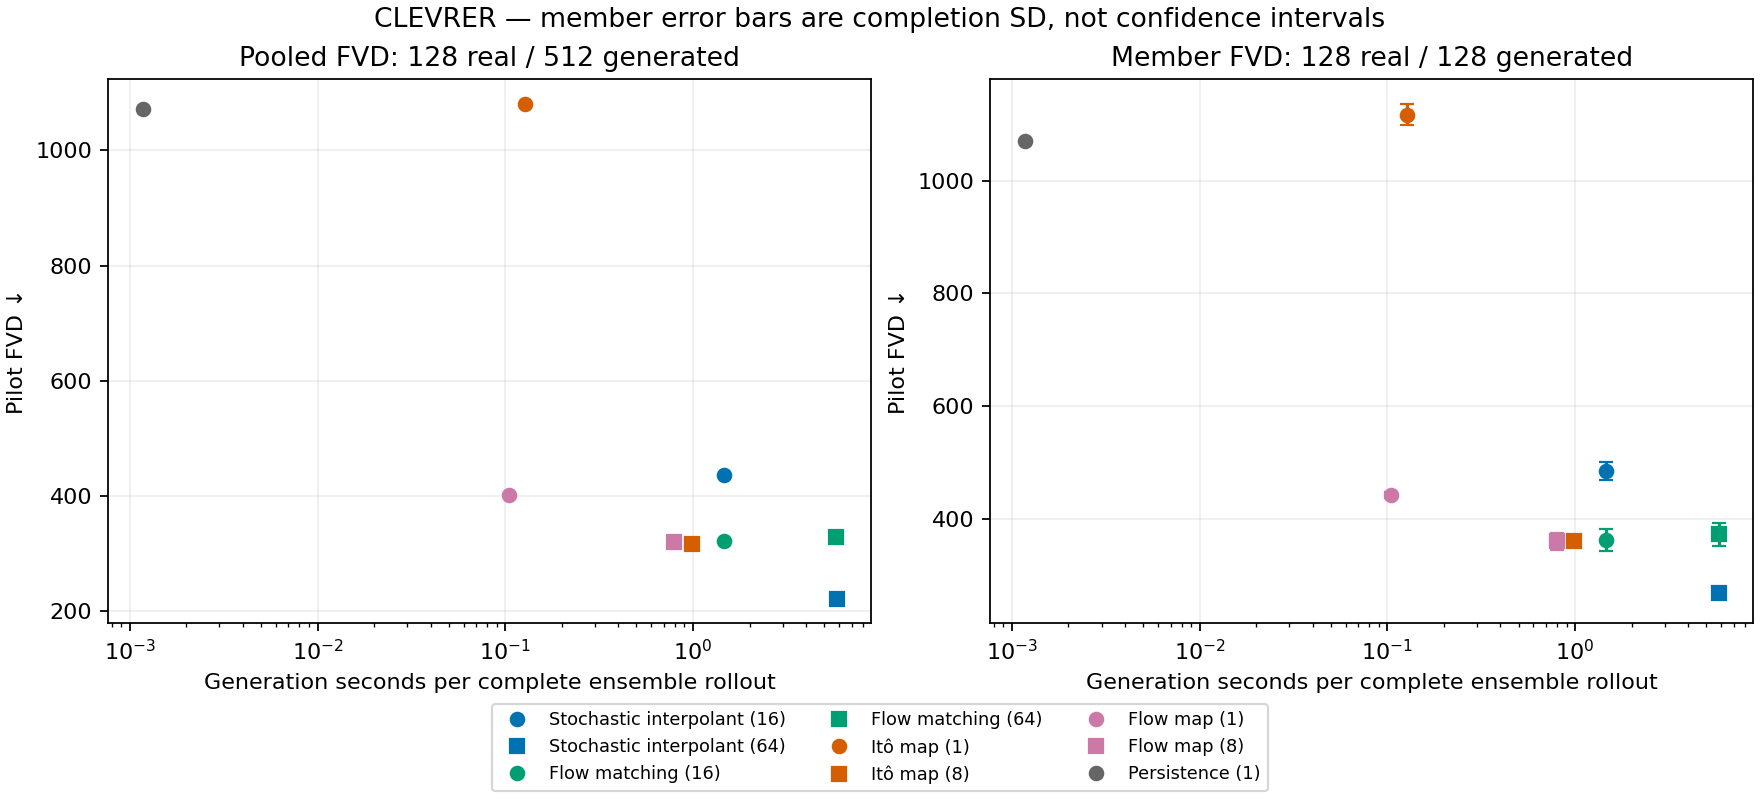
\includegraphics[width=\textwidth]{figures/video_results/clevrer_fvd_vs_cost.png}

\caption{CLEVRER: quality versus complete-ensemble generation cost, copied from the audited report without re-aggregating scores. The right panel uses equal-count member FVD; error bars are completion SD, not confidence intervals.}\label{fig:video-clevrer-cost}

\end{figure*}

\begin{figure*}[t]\centering

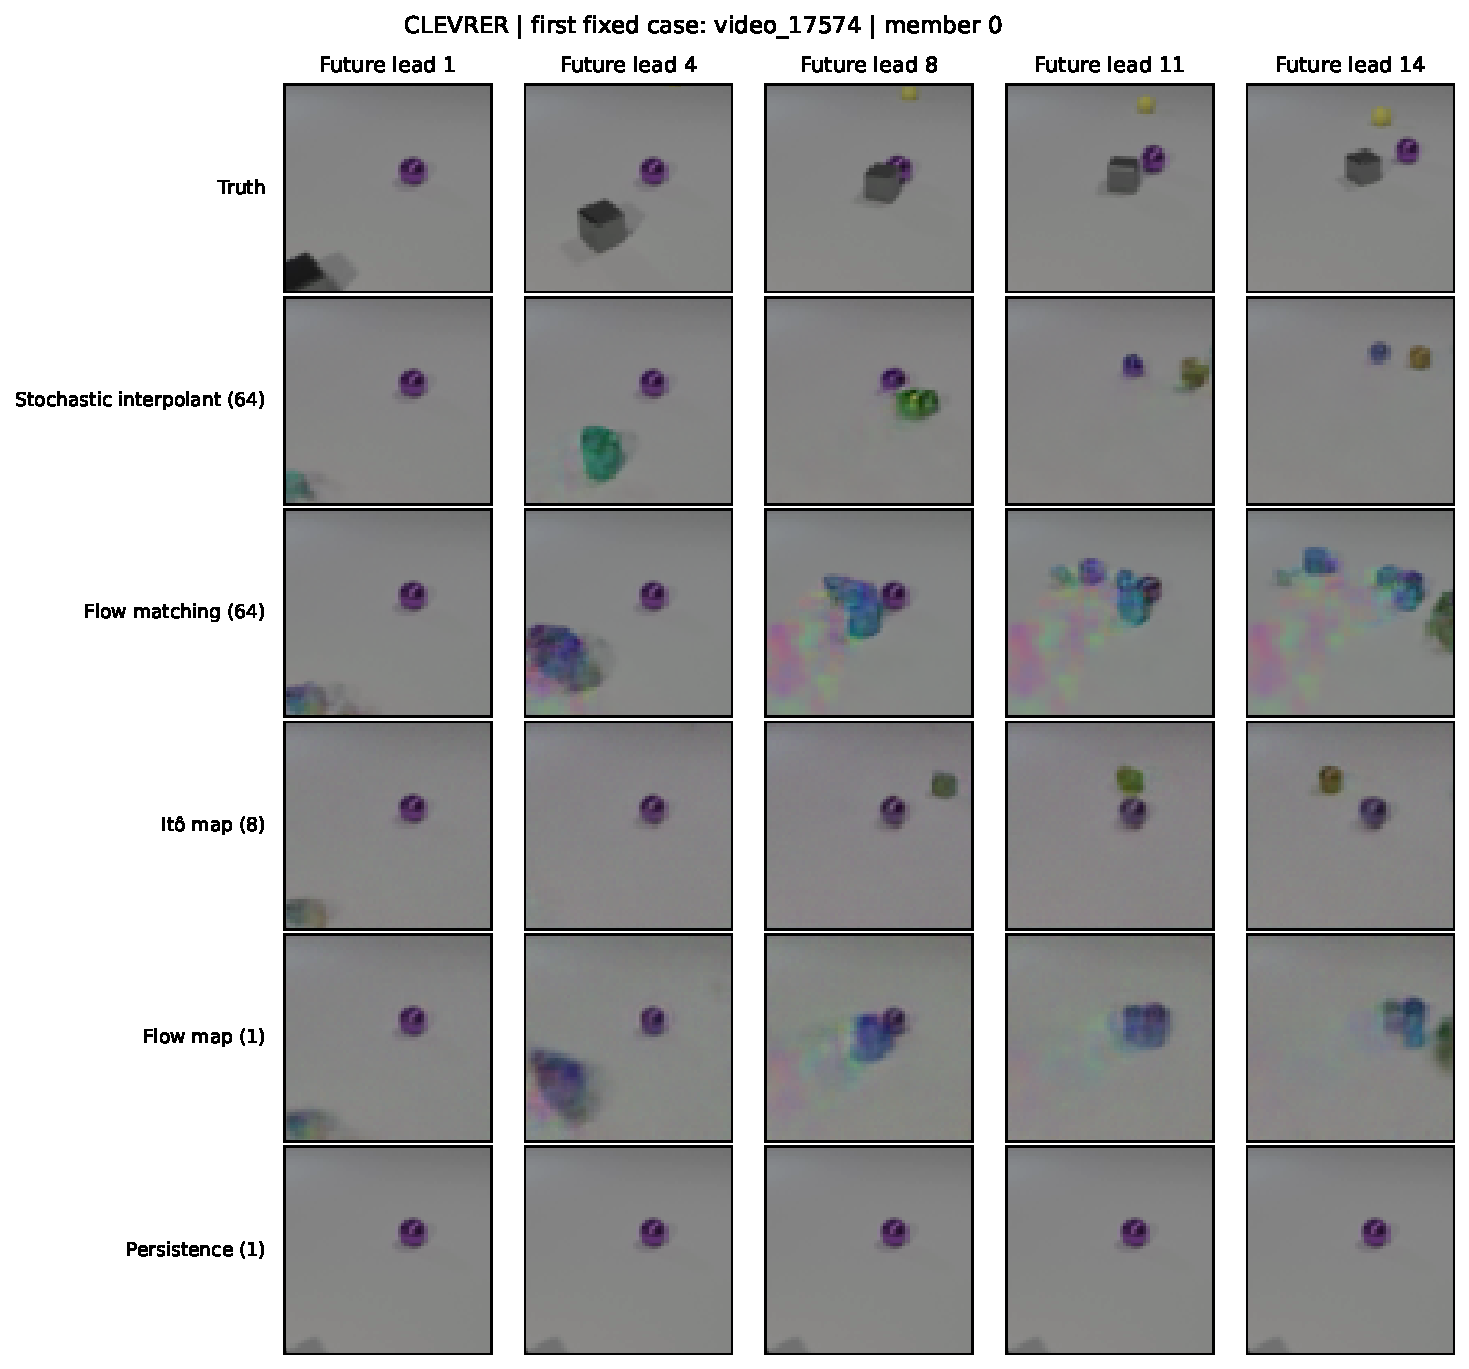
\includegraphics[width=\textwidth,height=.78\textheight,keepaspectratio]{figures/video_results/clevrer_fixed_forecast.pdf}

\caption{CLEVRER: the first preselected test case and ensemble member zero, at fixed future leads. Solver64, It\^o-map8, flow-map1 and persistence budgets were chosen before completed comparisons. All rows share the same observations and truth; no case or member was chosen by forecast quality. Display clips copies to the pixel range.}\label{fig:video-clevrer-forecast}

\end{figure*}

\begin{table*}[t]\centering\small

\begin{tabular}{lrrrrrr}
\toprule
Model & Steps/frame & Rollout NFE & Time (s)$\downarrow$ & CRPS$\downarrow$ & FVD pooled$\downarrow$ & FVD member mean $\pm$ SD \\
\midrule
SI & 16 & 480 & 3.07 & 0.0526 & 1781.7 & 1812.6 $\pm$ 16.3 \\
SI & 64 & 1920 & 12.58 & 0.0285 & 773.5 & 823.0 $\pm$ 20.7 \\
FM & 16 & 480 & 3.12 & 0.0265 & 726.8 & 766.9 $\pm$ 17.2 \\
FM & 64 & 1920 & 12.36 & 0.0264 & 783.1 & 831.5 $\pm$ 21.7 \\
It\^o map & 1 & 30 & 0.28 & 0.0319 & 1271.3 & 1302.2 $\pm$ 18.8 \\
It\^o map & 8 & 240 & 2.07 & 0.0286 & 888.2 & 926.5 $\pm$ 21.1 \\
Flow map & 1 & 30 & 0.23 & 0.0276 & 857.2 & 895.1 $\pm$ 18.1 \\
Flow map & 8 & 240 & 1.67 & 0.0277 & 706.6 & 748.0 $\pm$ 19.0 \\
Persistence & 1 & 0 & 0.00 & 0.0311 & 816.1 & 815.8 $\pm$ 0.0 \\
\bottomrule
\end{tabular}


\caption{KTH: matched pilot distributional quality and generation cost. Pooled FVD uses 128 real and 512 generated clips; member FVD uses 4 separate 128-versus-128 comparisons. Lower CRPS and FVD are better. Persistence has zero neural evaluations.}\label{tab:video-kth-quality}

\end{table*}

\begin{table*}[t]\centering\small

\begin{tabular}{lrrrrrr}
\toprule
Model & Steps/frame & Sample PSNR$\uparrow$ & Sample SSIM$\uparrow$ & Sample LPIPS$\downarrow$ & Mean PSNR$\uparrow$ & Mean SSIM$\uparrow$ \\
\midrule
SI & 16 & 20.55 & 0.480 & 0.377 & 21.46 & 0.626 \\
SI & 64 & 23.74 & 0.735 & 0.171 & 24.87 & 0.779 \\
FM & 16 & 24.30 & 0.769 & 0.163 & 25.25 & 0.790 \\
FM & 64 & 23.72 & 0.749 & 0.165 & 24.92 & 0.777 \\
It\^o map & 1 & 22.25 & 0.486 & 0.349 & 23.73 & 0.660 \\
It\^o map & 8 & 23.42 & 0.706 & 0.193 & 24.56 & 0.755 \\
Flow map & 1 & 24.23 & 0.733 & 0.191 & 25.01 & 0.777 \\
Flow map & 8 & 23.98 & 0.757 & 0.168 & 25.02 & 0.781 \\
Persistence & 1 & 24.77 & 0.805 & 0.165 & 24.77 & 0.805 \\
\bottomrule
\end{tabular}


\caption{KTH: future image quality, averaged across leads. Sample metrics average over completions. Mean PSNR/SSIM score the ensemble-mean image. Image/perceptual metrics use clipped copies; neither feedback nor proper scores are clipped.}\label{tab:video-kth-images}

\end{table*}

\begin{table*}[t]\centering\small

\begin{tabular}{lrrrrrrr}
\toprule
Model & Steps/frame & Energy$\downarrow$ & RMSE$\downarrow$ & RMS spread & Spread/skill & Coverage (\%) & Out of range (\%) \\
\midrule
SI & 16 & 0.0730 & 0.0968 & 0.0452 & 0.612 & 40.3 & 0.0 \\
SI & 64 & 0.0466 & 0.0653 & 0.0380 & 0.717 & 39.2 & 0.0 \\
FM & 16 & 0.0461 & 0.0632 & 0.0348 & 0.662 & 31.4 & 0.2 \\
FM & 64 & 0.0458 & 0.0654 & 0.0415 & 0.760 & 34.2 & 0.2 \\
It\^o map & 1 & 0.0504 & 0.0729 & 0.0483 & 0.828 & 59.1 & 0.2 \\
It\^o map & 8 & 0.0477 & 0.0673 & 0.0410 & 0.714 & 46.5 & 0.3 \\
Flow map & 1 & 0.0481 & 0.0639 & 0.0306 & 0.575 & 41.2 & 0.0 \\
Flow map & 8 & 0.0467 & 0.0648 & 0.0376 & 0.691 & 31.8 & 0.3 \\
Persistence & 1 & 0.0674 & 0.0674 & 0.0000 & 0.000 & 18.7 & 0.0 \\
\bottomrule
\end{tabular}


\caption{KTH: additional future-only proper-score and calibration diagnostics. Spread/skill includes the finite-ensemble correction; 90\% denotes the empirical central interval from four members and is not expected to attain 90\% even under ideal calibration. Out-of-range values are measured before display clipping.}\label{tab:video-kth-calibration}

\end{table*}

\begin{figure*}[t]\centering

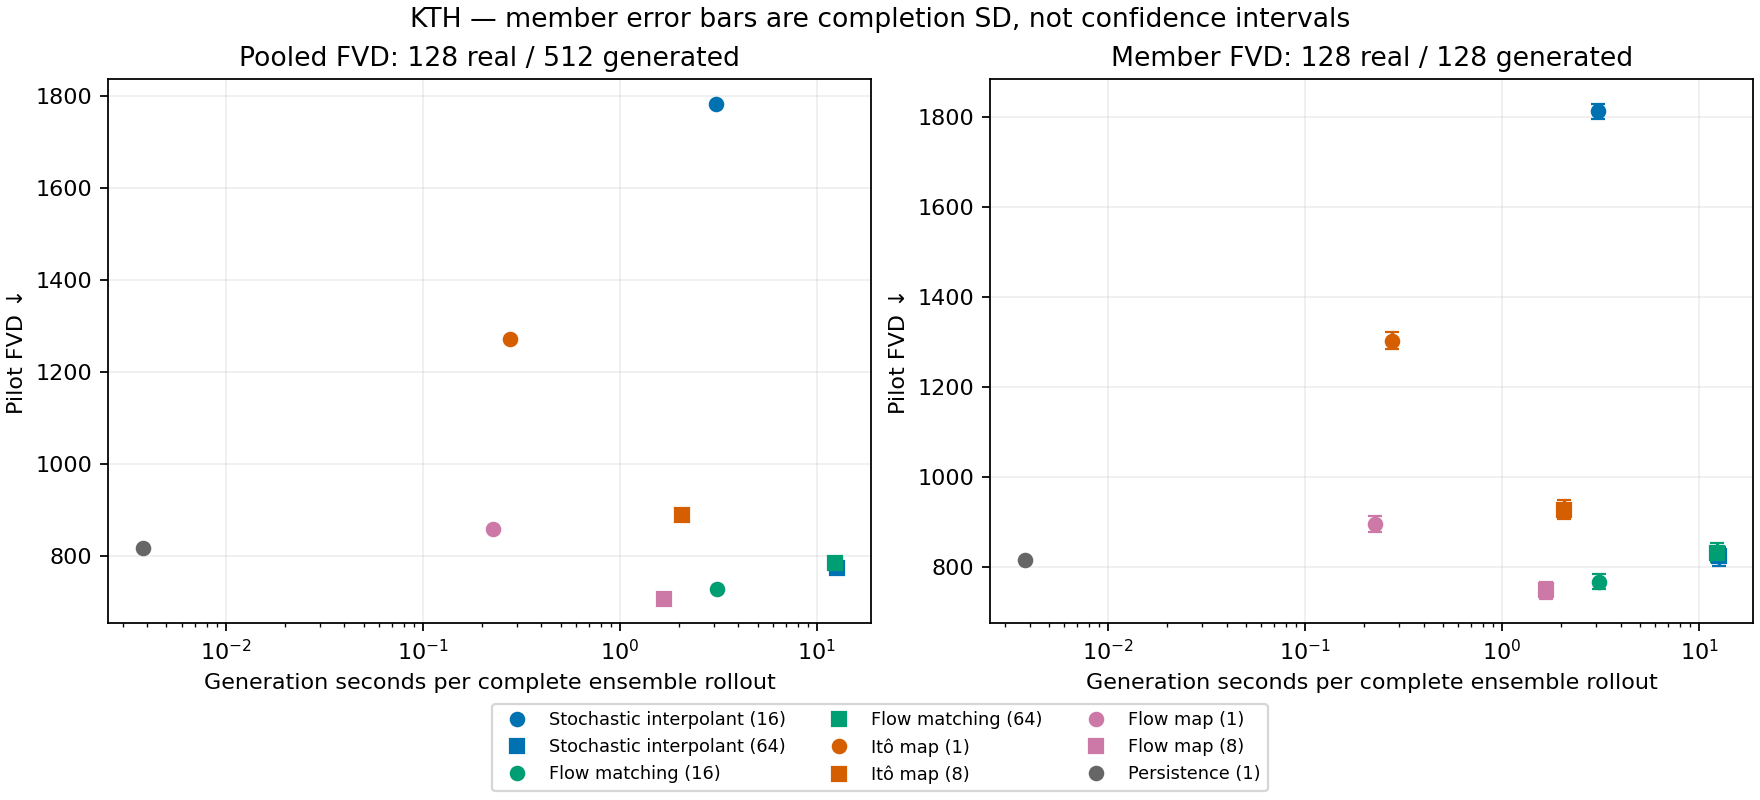
\includegraphics[width=\textwidth]{figures/video_results/kth_fvd_vs_cost.png}

\caption{KTH: quality versus complete-ensemble generation cost, copied from the audited report without re-aggregating scores. The right panel uses equal-count member FVD; error bars are completion SD, not confidence intervals.}\label{fig:video-kth-cost}

\end{figure*}

\begin{figure*}[t]\centering

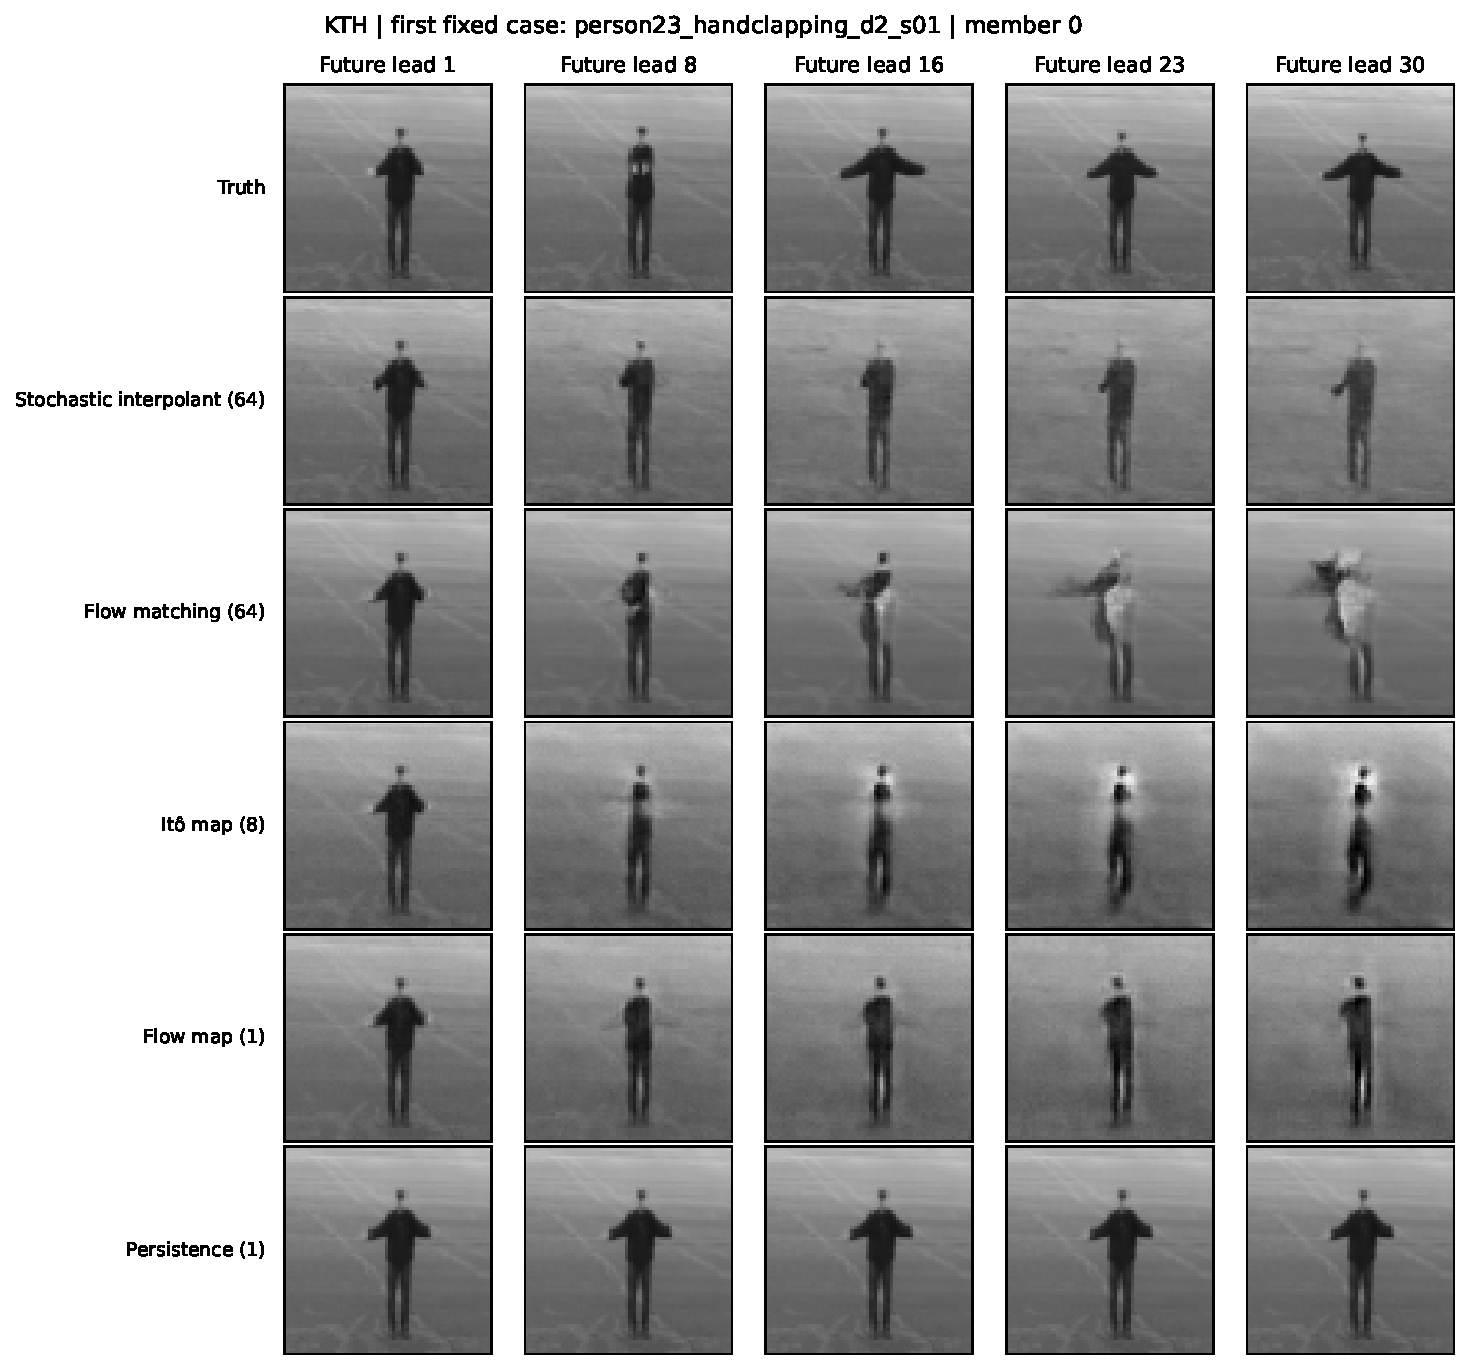
\includegraphics[width=\textwidth,height=.78\textheight,keepaspectratio]{figures/video_results/kth_fixed_forecast.pdf}

\caption{KTH: the first preselected test case and ensemble member zero, at fixed future leads. Solver64, It\^o-map8, flow-map1 and persistence budgets were chosen before completed comparisons. All rows share the same observations and truth; no case or member was chosen by forecast quality. Display clips copies to the pixel range.}\label{fig:video-kth-forecast}

\end{figure*}

Full per-lead source-video bootstrap intervals, additional oracle-member metrics and the unrounded aggregate metrics remain in the accompanying machine-readable reports. These intervals do not quantify training-seed variation. The finite-member forecast examples are illustrative rather than evidence of calibrated conditional uncertainty.
%
\paragraph{Reading the metrics together.}
The primary video endpoint is FVD, but the future-frame diagnostics expose different errors. The eight-step It\^o map has worse CRPS, energy score and mean sample LPIPS than SI64 on both datasets, although the KTH CRPS difference is small. The deterministic eight-step map improves FVD over FM64 while worsening CRPS and energy score on both datasets. Its mean sample LPIPS is also slightly worse. Thus a favorable sequence-feature distance need not imply better conditional scores or frame fidelity.

Persistence emphasizes this distinction: its energy score is worse than every learned CLEVRER configuration despite having the highest PSNR and SSIM and lowest sample LPIPS. Its images remain unchanged, so these strong frame-similarity values do not demonstrate plausible future motion. The displayed cases show actual sampled members and visible pose, texture and object differences; they are fixed examples rather than evidence of population-level ranking. Oracle best-member image metrics in the accompanying reports describe retrospective selection with knowledge of truth and must not be confused with average-completion performance.

Calibration diagnostics also require care. On CLEVRER, persistence has zero spread but empirical interval coverage of 80.8\%: its zero-width interval includes exactly unchanged pixels. Quantized values and ties invalidate the continuous-rank coverage bounds as literal targets for this dataset; high empirical pixel coverage alone does not certify uncertain-motion forecasting. Conversely, the one-step It\^o model has corrected spread/skill near one (1.027), yet poor FVD (1080.0). Matching an aggregate second-moment ratio does not establish the right spatial or temporal distribution. The eight-step It\^o ratios are 0.714 on KTH and 0.780 on CLEVRER, versus 0.717 and 0.877 for SI64; these are averages of context-level ratios, not proofs of conditional calibration.

All image metrics use clipped copies and all proper scores retain original predictions. Mean out-of-range fractions are small but not identically zero: the largest is about 0.34\% for KTH FlowMap8. The fixed-size FVD estimates, source-video-weighted frame scores and four-member uncertainty diagnostics measure different aspects of this particular pilot. No paired FVD significance test or training-seed uncertainty estimate is provided, and completion SD must not be read as either.
%
}{%
\paragraph{Current status.}
Evaluation is in progress. Tables~\ref{tab:video-setup}--\ref{tab:video-training} and Figure~\ref{fig:video-dataset-preview} document the completed setup; no video forecast-quality or acceleration claim is made at this stage. The complete matched comparison will be included after both datasets pass artifact verification.
}
